\section{Diagrammi di attività}
	\subsection{Diagrammi di attività utente}
		\subsubsection{Login}
		\begin{center}
			\begin{figure}[htbp]
				\centering
				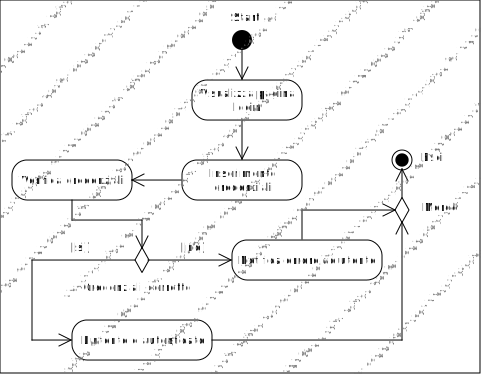
\includegraphics[scale=0.8]{\docsImg /immagini.diagrammi/Login.pdf}
			\caption{DA 1 - La procedura di Login.}	
			\end{figure}
		\end{center}
		\noindent \textbf{Descrizione: }l'utente visualizza la pagina di login ed inserisce le proprie credenziali. Le credenziali inserite vengono verificate. Se queste sono corrette l'utente diviene autenticato e la sequenza di attività termina, altrimenti gli viene notificato l'errore di autenticazione e la sequenza di attività termina.
		\newpage
		
		
		
		\subsubsection{Registrazione}
		\begin{center}
			\begin{figure}[htbp]
				\centering
				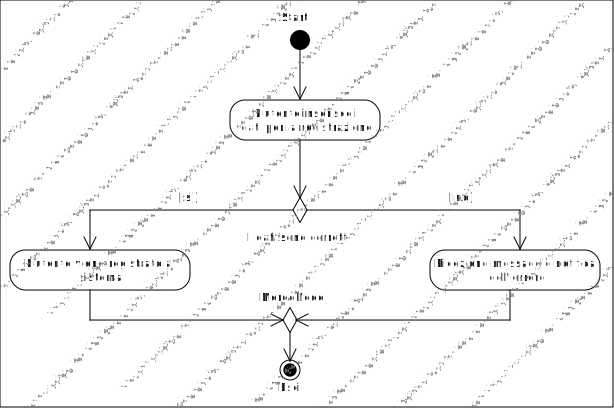
\includegraphics[scale=0.8]{\docsImg /immagini.diagrammi/Registrazione.pdf}
			\caption{DA 2 - La procedura di Registrazione.}	
			\end{figure}
		\end{center}
		\noindent \textbf{Descrizione: }l'utente si vuole registrare al servizio, viene visualizzato il form per la registrazione e l'utente inserisce i propri dati. Se i dati sono corretti (soddisfano quindi le condizioni poste in fase di analisi dei requisiti), il sistema procede con la registrazione del nuovo utente e la sequenza di attività termina, altrimenti l'utente riceve un opportuno messaggio che descrive la natura dell'errore e la sequenza di attività termina.
		\newpage
		
		
		
		\subsubsection{Modifica dati}
		\begin{center}
			\begin{figure}[htbp]
				\centering
				\includegraphics[scale=0.8]{\docsImg /immagini.diagrammi/ModificaDatiUtente.pdf}
			\caption{DA 3 - La procedura di modifica dei dati dell'utente.}	
			\end{figure}
		\end{center}		
		\noindent \textbf{Descrizione: }l'utente visualizza i propri dati, seleziona il dato che vuole modificare e inserisce il nuovo dato. \newline Se il dato modificato non è la mail il sistema procede con la modifica e la sequenza di attività termina. \newline Se il dato modificato è la mail il sistema comunica con il server\g~ per controllare la sua correttezza secondo le norme stabilite in analisi dei requisiti. Il sistema attende la risposta del server\g~ in merito al controllo di unicità. Se la mail è univoca allora il sistema procede con la modifica e la sequenza di attività termina, altrimenti la richiesta di modifica non viene eseguita e il sistema riporta un opportuno messaggio di errore all'utente e la sequenza di attività termina.
		\newpage
		
		
		
		\subsubsection{Ricevimento chiamata}
		\begin{center}
			\begin{figure}[htbp]
				\centering
				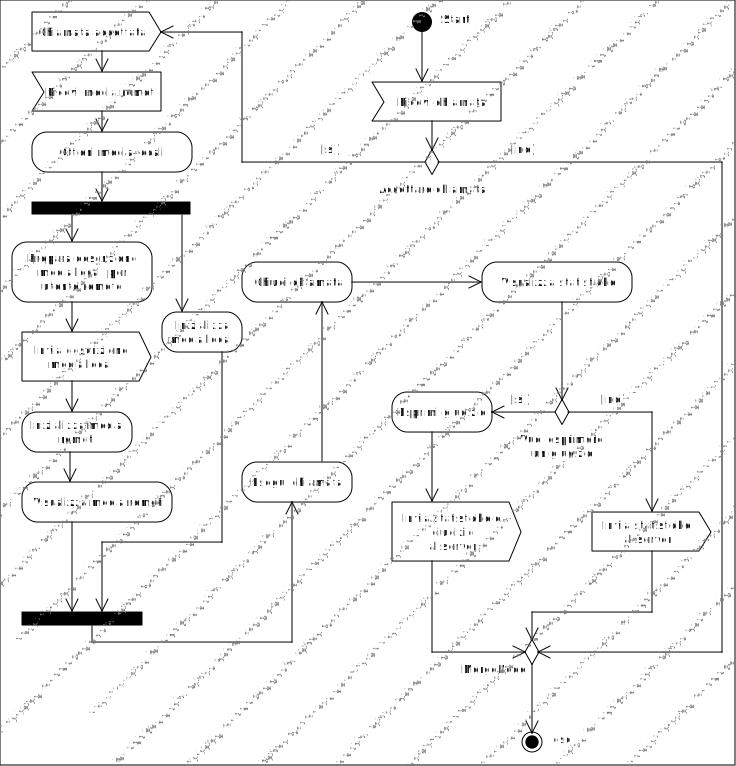
\includegraphics[scale=0.8]{\docsImg /immagini.diagrammi/ReceiveCall.pdf}
			\caption{DA 4 - La procedura di ricezione di una chiamata.}	
			\end{figure}
		\end{center}		
		\noindent \textbf{Descrizione: }l'utente riceve una notifica dal sistema di una chiamata in arrivo che può essere accettata o rifiutata. Nel caso la chiamata venga rifiutata, l'utente esce dalla fase di gestione della chiamata in arrivo e la sequenza di attività termina. Se, invece, l'utente accetta la chiamata avvengono le seguenti operazioni:
		\begin{enumerate}
			\item l'utente ha accettato la chiamata ed invia il segnale di accettazione al mittente; 
			\item l'utente riceve dal mittente la descrizione della sessione remota (media remoti);
			\item il sistema richiede all'utente l'accesso ai media locali (gestito dal browser$_{|g|}$);
			\item si eseguono in parallelo due sequenze di attività. La prima:
				\begin{enumerate}
					\item si prepara la descrizione della sessione locale da inviare all'utente remoto che poi provvederà a gestirla opportunamente; 
					\item si invia tale descrizione attraverso il server\g~ all'utente remoto, senza attendere alcuna risposta;
					\item si ricevono i candidati ICE;
					\item si inizializzano e si visualizzano i media remoti all'interno della pagina web$_{|g|}$.
				\end{enumerate}
			La seconda:
			\begin{enumerate}
			 	\item si inizializzano e si visualizzano i media locali all'interno della pagina web$_{|g|}$.
			\end{enumerate}
		\end{enumerate} 
		Quando tutte queste attività sono terminate la chiamata è iniziata ed è possibile per gli utenti comunicare in tempo reale. 
		Viene allora eseguita la chiamata, che continua fino a quando uno dei due utenti non decide di terminare la chiamata.
		Vengono quindi visualizzate dall'utente le statistiche relative alla chiamata appena conclusa. All'utente viene richiesto di esprimere un giudizio in merito alla qualità della chiamata. Se l'utente accetta, esprime il giudizio e vengono inviate al server$_{|g|}$ le statistiche e il giudizio e, senza attendere alcuna risposta, la sequenza di attività termina. Se invece rifiuta vengono inviate al server$_{|g|}$ le statistiche e, senza attendere alcuna risposta, la sequenza di attività termina.
		\newpage
		
		
		
		\subsubsection{Chiama inserendo dato}
		\begin{center}
			\begin{figure}[htbp]
				\centering
				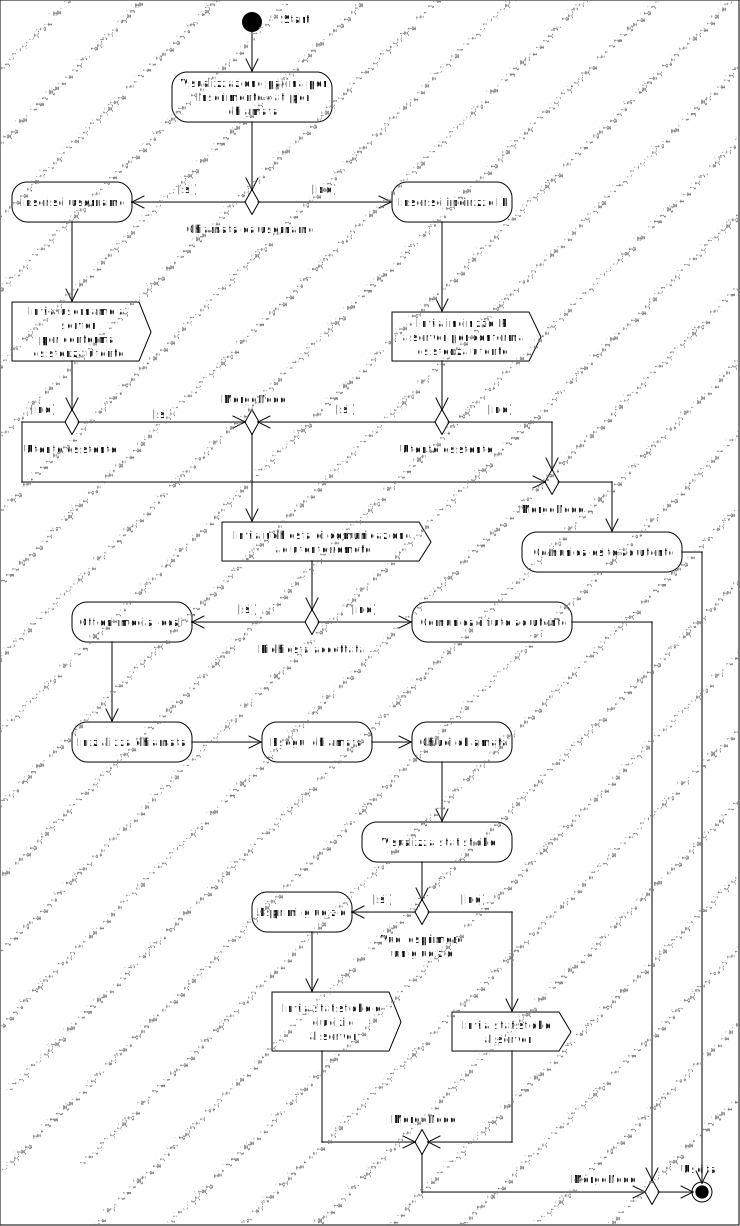
\includegraphics[scale=0.65]{\docsImg /immagini.diagrammi/MakeCallInsertData.pdf}
			\caption{DA 5 - La procedura di chiamata inserendo un dato conosciuto (username o indirizzo IP).}	
			\end{figure}
		\end{center}		
		\noindent \textbf{Descrizione: }l'utente sceglie di chiamare un altro utente tramite lo username o l'indirizzo IP$_{|g|}$ e visualizza la pagina per l'inserimento di tale dato.
		L'utente inserisce lo username o l'indirizzo IP$_{|g|}$ dell'utente da chiamare. Il sistema invia il dato inserito al server\g~ per avere la conferma dell'esistenza dell'utente ed attende la risposta.
		Se l'utente non esiste il sistema notifica l'esito negativo e la sequenza delle attività termina.
		Se l'utente esiste, gli viene inviata una richiesta di comunicazione e il sistema attende una risposta. Se la richiesta viene rifiutata l'utente che ha inviato la richiesta riceve debita comunicazione e la sequenza di attività termina.
		Se la richiesta viene accettata avviene la seguente sequenza di operazioni:
		\begin{enumerate}
			\item viene chiesto all'utente di accedere ai media locali (\textit{es.} webcam e microfono);
			\item la chiamata viene inizializzata, eseguita e successivamente terminata;
			\item vengono mostrate all'utente le statistiche sulla chiamata appena terminata;
			\item viene richiesto all'utente di esprimere un giudizio in merito alla qualità della chiamata:
			\begin{itemize}
			\item se l'utente accetta, esprime il giudizio e vengono inviate al server$_{|g|}$ le statistiche e il giudizio e, senza attendere alcuna risposta, la sequenza di attività termina;
			\item se invece rifiuta vengono inviate al server$_{|g|}$ le statistiche e, senza attendere alcuna risposta, la sequenza di attività termina.
			\end{itemize}
		\end{enumerate}
		\newpage
		
		
		
		\subsubsection{Chiama selezionando da lista}
		\begin{center}
			\begin{figure}[htbp]
				\centering
				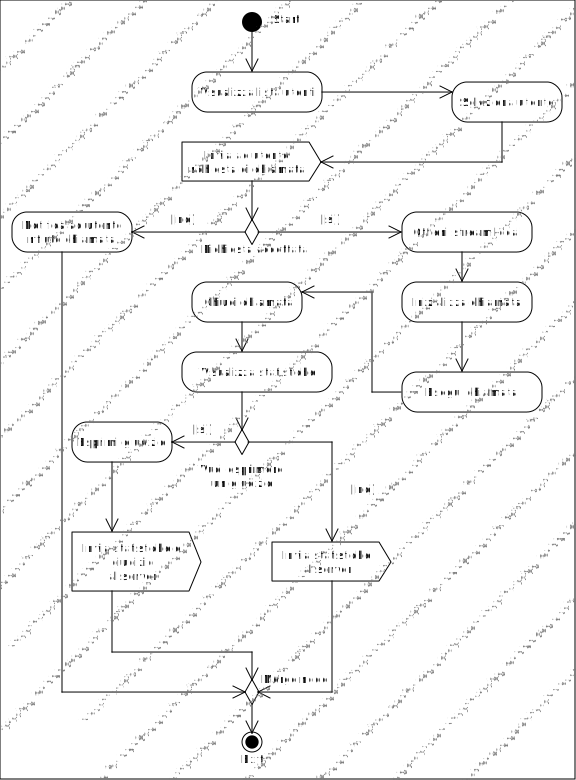
\includegraphics[scale=0.7]{\docsImg /immagini.diagrammi/MakeCallList.pdf}
			\caption{DA 6 - La procedura di effettuazione di una chiamata dalla lista.}	
			\end{figure}
		\end{center}		
		\noindent \textbf{Descrizione: }l'utente visualizza la lista degli utenti registrati al server$_{|g|}$ e seleziona l'utente che desidera chiamare.
		Il sistema invia all'utente selezionato una richiesta di chiamata e attende la risposta.
		Se la chiamata viene rifiutata, viene notificato all'utente il rifiuto da parte del destinatario e la sequenza delle attività termina.
		Se la chiamata viene accettata avviene la seguente sequenza di operazioni:
		\begin{enumerate}
			\item si ottiene l'accesso ai media locali;
			\item la chiamata viene inizializzata, eseguita ed infine chiusa;
			\item vengono mostrate all'utente le statistiche sulla chiamata appena terminata;
			\item viene richiesto all'utente di esprimere un giudizio in merito alla qualità della chiamata:
			\begin{itemize}
			\item se l'utente accetta, esprime il giudizio e vengono inviate al server$_{|g|}$ le statistiche e il giudizio e, senza attendere alcuna risposta, la sequenza di attività termina;
			\item se invece rifiuta vengono inviate al server$_{|g|}$ le statistiche e, senza attendere alcuna risposta, la sequenza di attività termina.
			\end{itemize}
		\end{enumerate}	

		
		
		
		\subsubsection{Inizializza chiamata}
		\begin{center}
			\begin{figure}[htbp]
				\centering
				\includegraphics[scale=0.8]{\docsImg /immagini.diagrammi/InizializzaChiamata.pdf}
			\caption{DA 6.1 - La procedura di inizializzazione di una chiamata.}	
			\end{figure}
		\end{center}
		\noindent \textbf{Descrizione: }una volta ottenuti i media locali si svolgono due sequenze di attività in parallelo. La prima:
		\begin{enumerate}
			\item si prepara la descrizione di media locali per l'utente remoto;
			\item la descrizione preparata al punto 1 viene inviata all'utente remoto;
			\item si attende come risposta dall'utente remoto la descrizione dei suoi media locali;
			\item si inviano i propri candidati ICE;
			\item si attende la ricezione dei candidati ICE remoti;
			\item al ricevimento della risposta del punto 5, l'utente locale inizializza i media remoti nella propria pagina.
		\end{enumerate}
		La seconda:
		\begin{enumerate}
			\item si inizializzano i media locali.
		\end{enumerate}
		Una volta che le due sequenze sono state completate, si ottiene un canale di comunicazione tra i due utenti che vogliono comunicare.

		
		
		
	\subsection{Diagrammi di attività amministratore}
	
		\subsubsection{Login}
		\begin{center}
			\begin{figure}[htbp]
				\centering
				\includegraphics[scale=0.8]{\docsImg /immagini.diagrammi/LoginAdmin.pdf}
			\caption{DA 7 - La procedura di inizializzazione di una chiamata.}	
			\end{figure}
		\end{center}
		\noindent \textbf{Descrizione: }l'utente amministratore visualizza la pagina di login ed inserisce le proprie credenziali. Le credenziali inserite vengono verificate. Se queste sono corrette l'utente amministratore diviene autenticato e la sequenza di attività termina, altrimenti gli viene notificato l'errore di autenticazione e la sequenza di attività termina.
		\newpage
		
		
		\subsubsection{Visualizzazione statistiche amministratore}
		\begin{center}
			\begin{figure}[htbp]
				\centering
				\includegraphics[scale=0.8]{\docsImg /immagini.diagrammi/Admin.pdf}
			\caption{DA 8 - La procedura di visualizzazione delle statistiche.}	
			\end{figure}
		\end{center}
		\noindent \textbf{Descrizione: }
		l'utente amministratore visualizza la sua pagina principale nella quale visualizza le statistiche relative alle comunicazioni effettuate, tra gli utenti registrati, nell'ultima settimana.
		L'amministratore ha la possibilità di filtrare queste chiamate. Se decide di non filtrarle, effettua il logout e la sequenza di attività termina.
		Se decide di filtrarle può farlo in base alla data di effettuazione, al giudizio ottenuto o all'utente che vi ha partecipato. Dopo aver applicato il filtro il sistema permette all'amministratore di visualizzare i risultati della ricerca. Infine l'amministratore effettua il logout e la sequenza di attività termina.

\newpage